\newpage
\section{Modelisation avec UML}

  Afin de faciliter l'implementation nous avons décider de modéliser
  notre application en utilisant la méthode UML. Pour cela nous nous
  sommes appuyés sur les connaissances aquises lors du module
  Ingénierie Logiciel du semestre précédent.

  \subsection{Cas d'utilisation}
  
    \begin{figure}[h!]
      \centering
      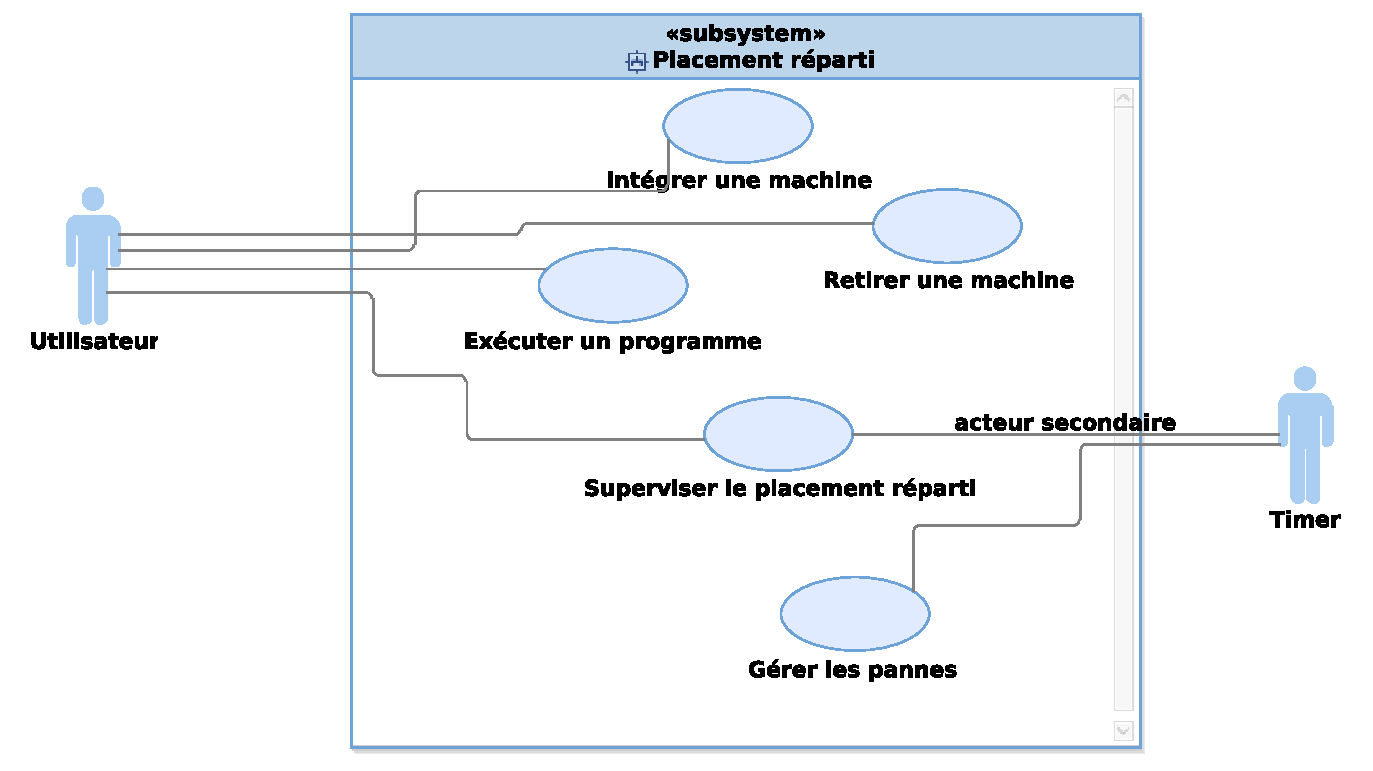
\includegraphics[width=\textwidth]{img/analyse_DiagrammeCasUtilisation.pdf}
      \caption{Diagramme de cas d'utilisation}
    \end{figure}
    
    \subsubsection{Liste des acteurs}

      \begin{tabular}{|l|p{5cm}|l|}
        \hline \bf Acteur & \bf Description & \bf Type \\ \hline
        Utilisateur & Personne qui utilise une machine intégrée au
        placement système de placement réparti & Primaire \\ \hline
        Temporisateur & Indicateur de problème interne au système & Primaire, Secondaire
        \\ \hline
      \end{tabular}
    
  \subsubsection{Liste des cas d'utilisation}
    \begin{tabular}{|l|p{7cm}|}
      \hline
        \bf Cas d'utilisation &
        \bf Description \\
      \hline
        Intégrer une machine &
        Permet à un utilisateur d'intégrer sa machine dans le système
        de placement réparti \\
      \hline
        Exécuter un programme &
        Permet à un utilisateur d'exécuter un programme dans le
        système \\
      \hline
        Superviser le placement &
        Il permet à un utilisateur de consultés l'ensemble des données
        du placement réparti : machines, charges et programmes exécutés
        à distance \\
      \hline
        Retirer une machine &
        Il permet à un utilisateur de retirer sa machine du placement 
        réparti \\
      \hline
        Gérer les pannes &
        Il permet à un Timer de vérifier périodique si une machine n'est
        pas en panne et de la gérer \\
      \hline
    \end{tabular}
  \newpage

  \subsubsection{Cas Éxécuter un programme}

    \begin{figure}[h!]
      \centering
      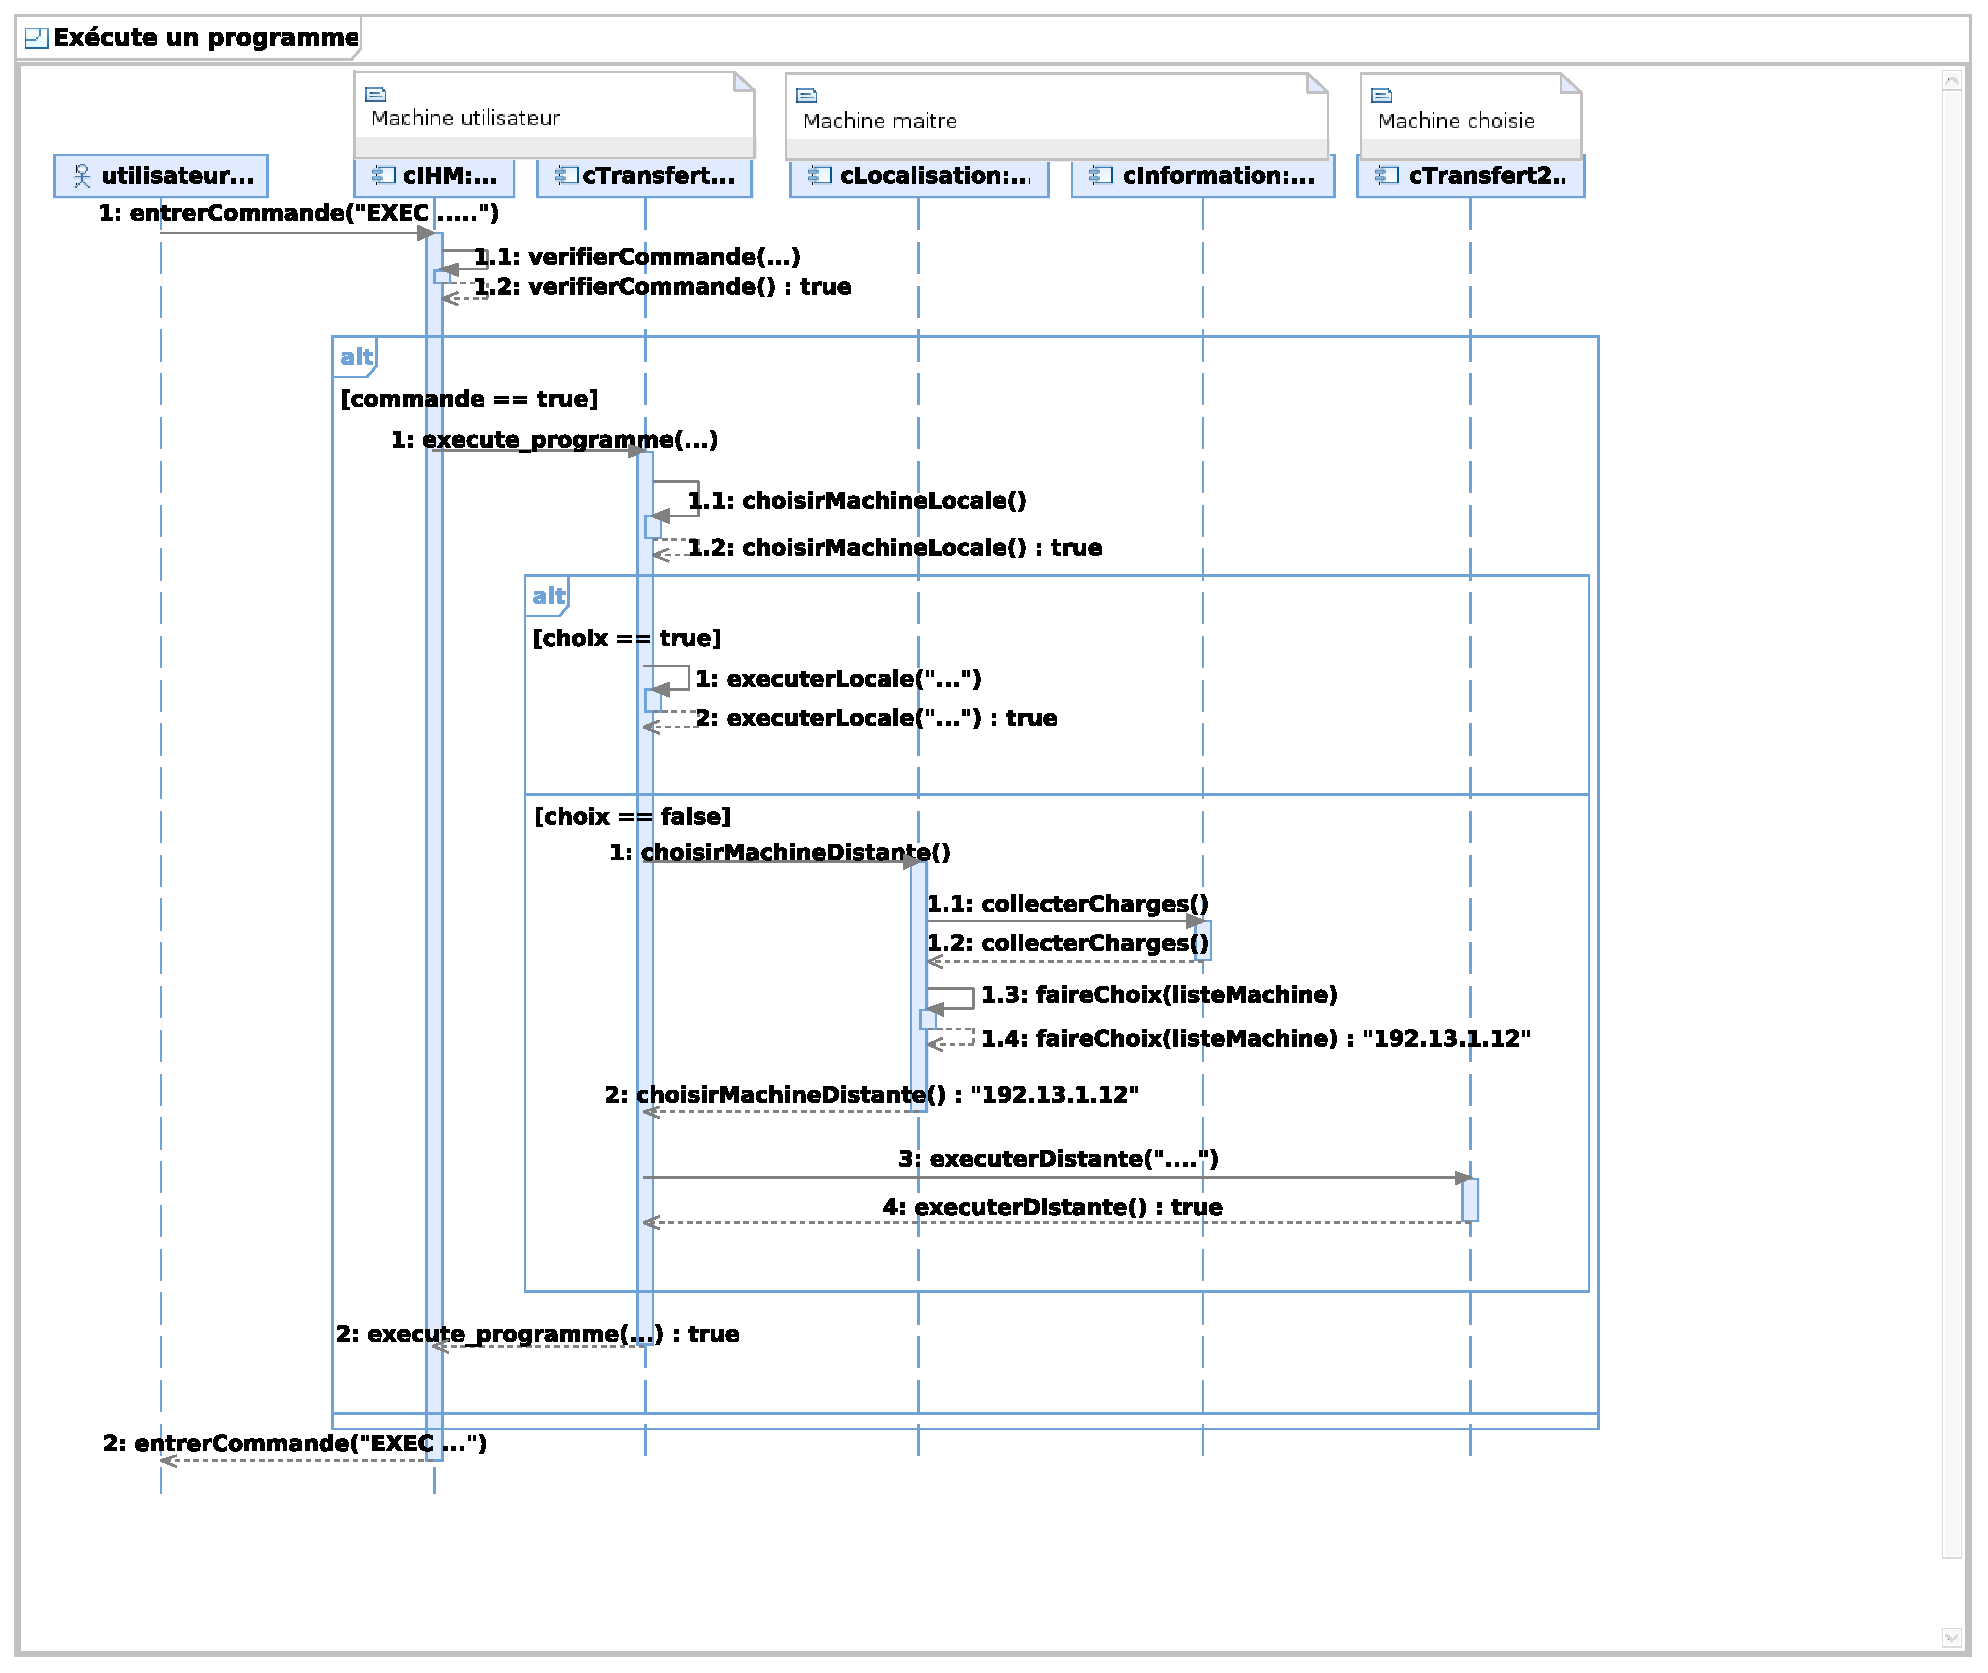
\includegraphics[width=\textwidth]{img/analyse_DSCexecprog.pdf}
      \caption{Diagramme de séquence -- Cas Éxecuter un programme}
    \end{figure}

    Description des étapes permettant à un utilisateur d'exécuter un
    programme au sein du système de répartition de tâches. \\
    
    \noindent
    {\bf Acteur principal} Utilisateur \\
    {\bf Acteur secondaire} Aucun \\
    {\bf Séquence} Le cas d'utilisation commence lorsque l'utilisateur
      lance son programme \\
    {\bf Pré-conditions} \hfill
    \begin{itemize}
      \item Le placement doit être fonctionnel
      \item La machine doit être intégrée au placement réparti
      %\item Le programme doit être un programme valide au placement
    \end{itemize}
        
    \paragraph{Scénario nominal} La machine choisie est celle de
      l'utilisateur où la commande est lancée.

      \begin{enumerate}
        \item L'utilisateur demande le placement d'une tâche
        \item Le système choisit une machine parmi les machines du
            placement pouvant accueillir le programme
        \item Le système exécute le programme sur la machine choisie et attend le résultat
        \item Le système informe le client de la terminaison de son programme
      \end{enumerate}

    \paragraph{Alternatives}
      \begin{description}
        \item[A1] La machine choisie est une machine distante
          \begin{enumerate}
            \setcounter{enumi}{2}
            \item Le système enregistre le programme et ses paramètres dans
                   sa liste des programmes exécutés à distance
            \item Le système exécute le programme sur la machine choisie et
                   attend le résultat
            \item Le système retire le programme et ses paramètres de sa
                   liste des programmes exécutés à distance
          \end{enumerate}

        %% \item[A2] Le programme ou les paramètres sont incorrects
        %%   L'enchainement démarre après le point 2 de la séquence
        %%   nominale

        %%   \begin{enumerate}
        %%     \setcounter{enumi}{2}
        %%     \item Le système indique à l'utilisateur que les données
        %%       entrées du programme sont incorrectes La séquence
        %%       nominale reprend au début
        %%   \end{enumerate}
      \end{description}

   \paragraph{Exceptions}
     \begin{description}
       \item[E1] L'exécution du programme est interrompu suite à un
         problème quelconque du programme
         \begin{enumerate}
           \setcounter{enumi}{3}
           \item Le système indique à l'utilisateur de l'interruption
             de son programme
         \end{enumerate}

       \item[E2] Problème de communication entre machine source et cible
         \begin{enumerate}
           \setcounter{enumi}{3}
           \item Après trois tentatives sans acquittement, le système
             abandonne (la suite sera gérée par la gestion de pannes)
          \end{enumerate}
     \end{description}

  \subsubsection{Cas Intégrer une machine}

    \begin{figure}[h!]
      \centering
      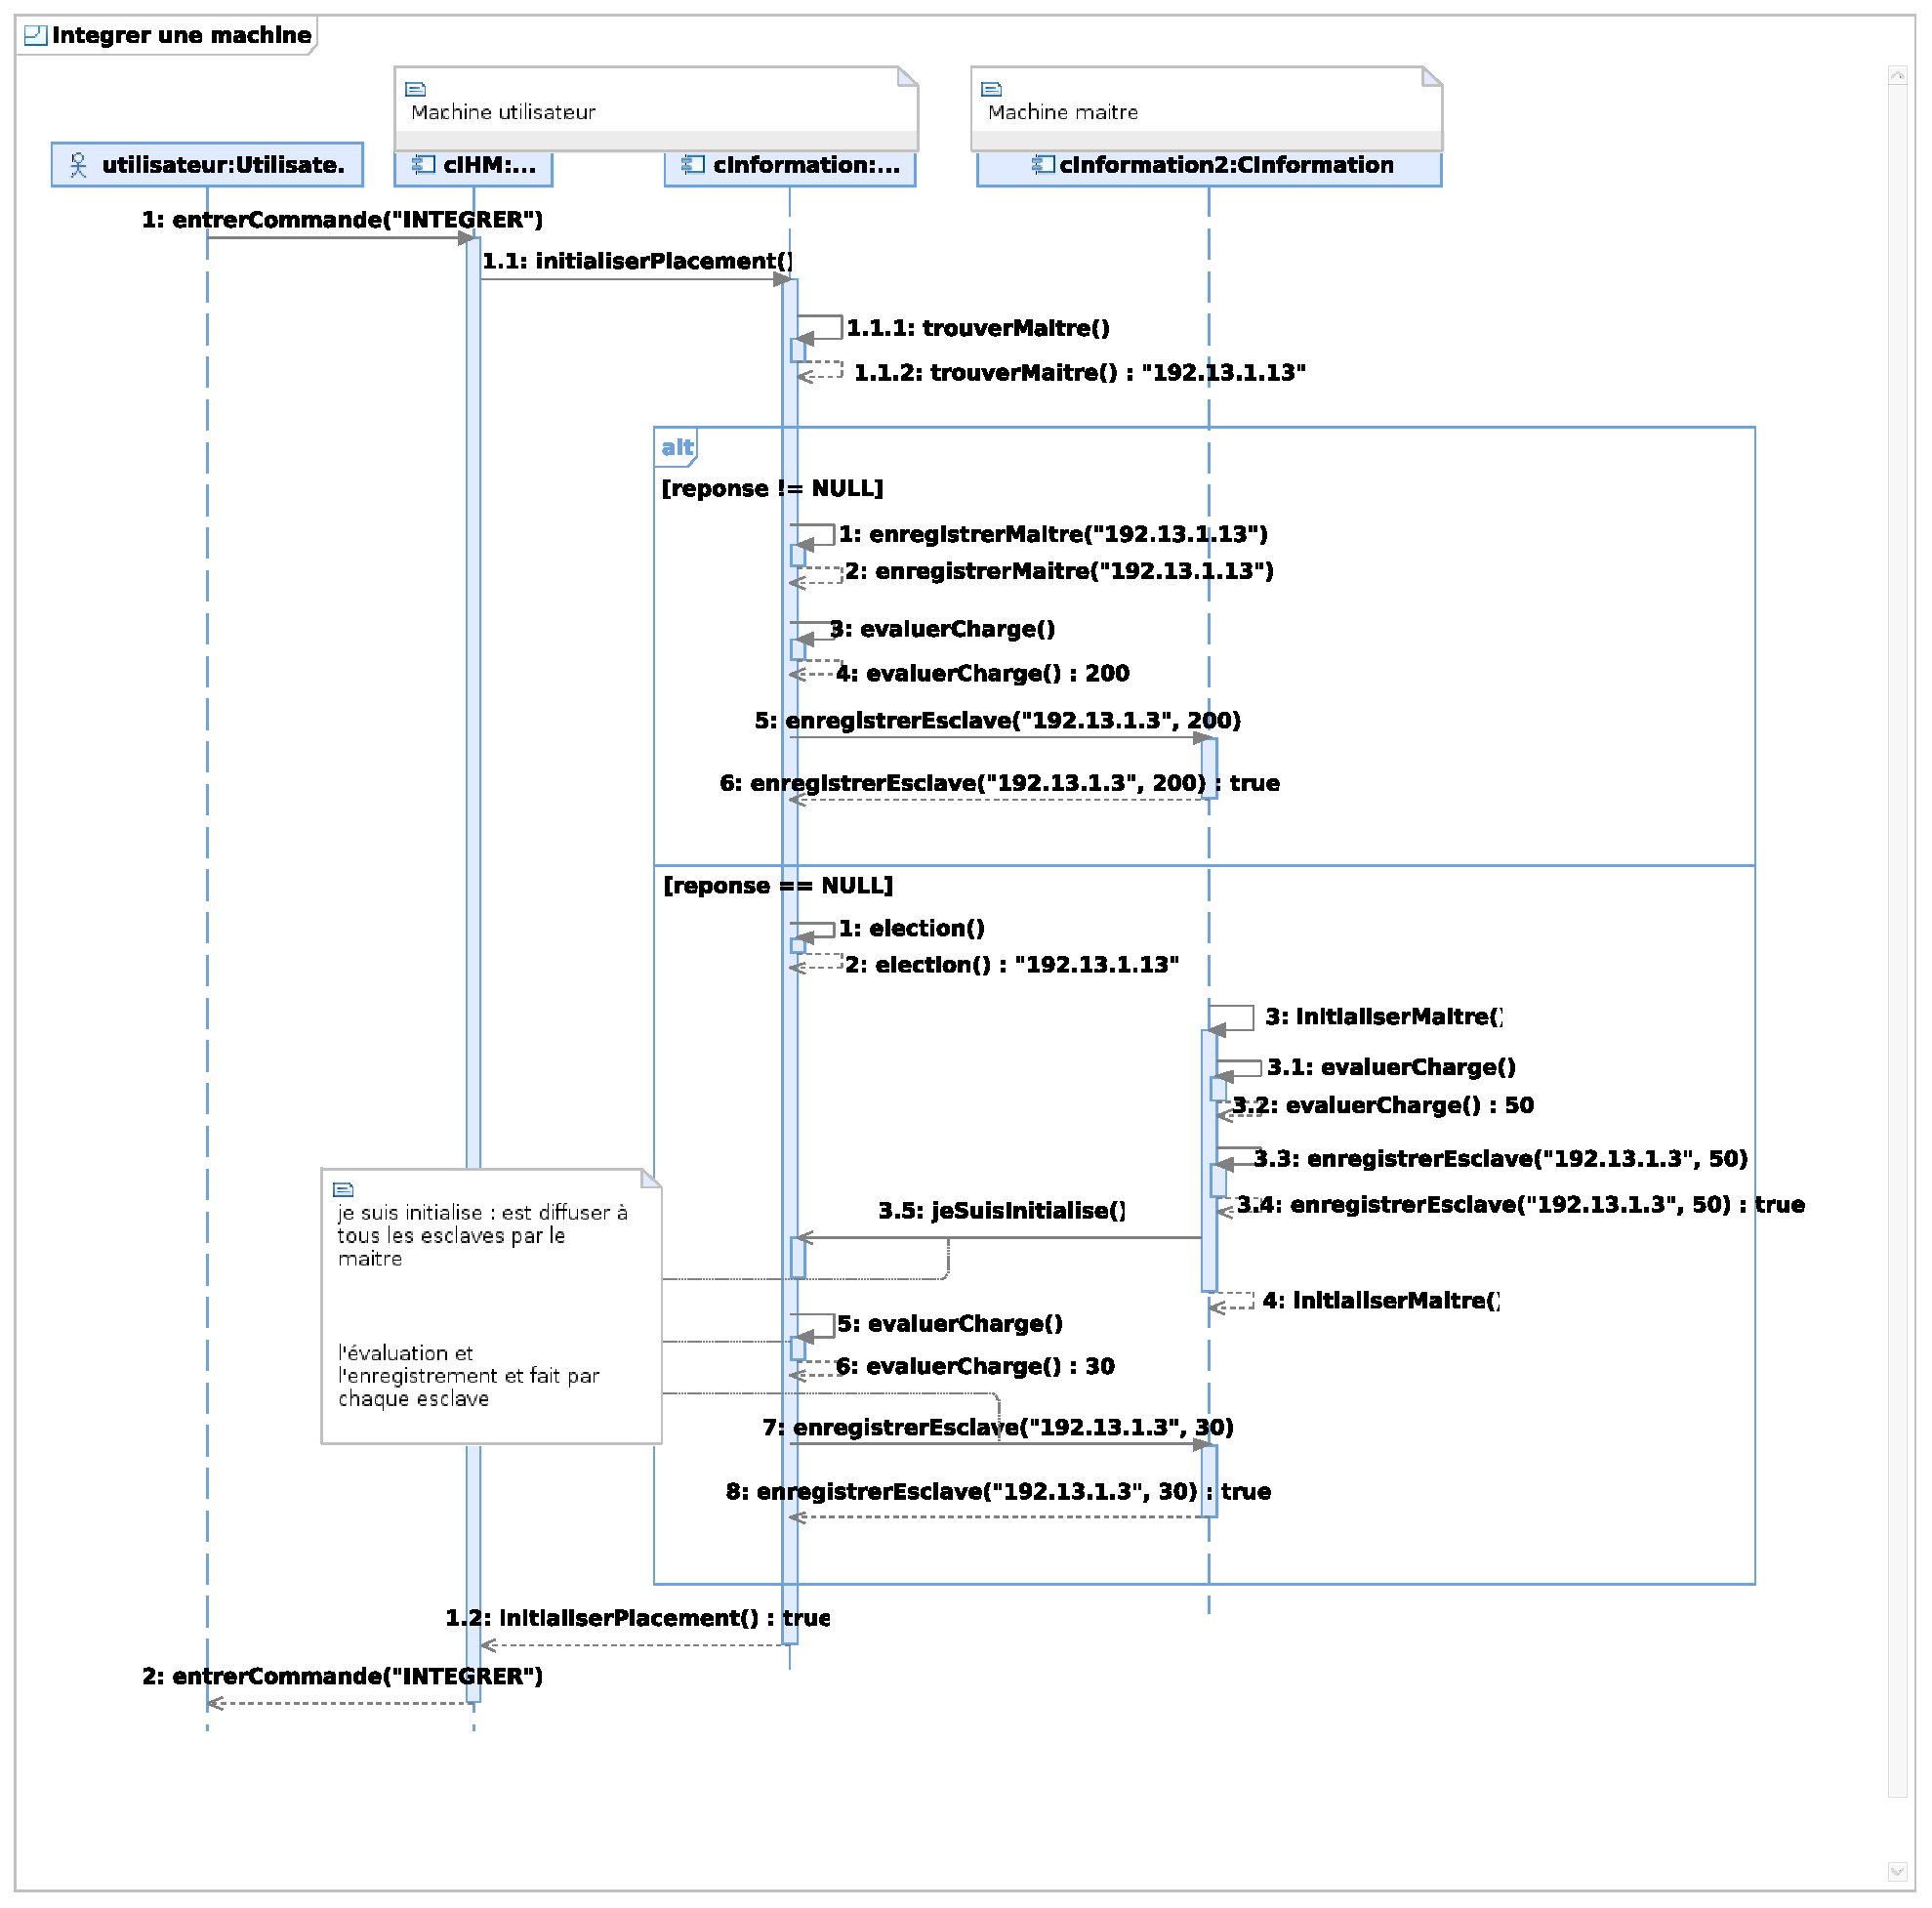
\includegraphics[width=\textwidth]{img/analyse_DSseqintegermach.pdf}
      \caption{Diagramme de séquence -- Cas Intégrer une machine}
    \end{figure}

    Description des étapes permettant à un utilisateur d'intégrer sa
    machine au placement réparti afin qu'elle puisse répartir ou
    recevoir des programmes. \\

    \noindent
    {\bf Acteur principal} Utilisateur \\
    {\bf Acteur secondaire} Aucun \\
    {\bf Séquence} Le cas d'utilisation commence lors du démarrage du
      service de placement réparti \\ 
    {\bf Pré-conditions} \hfill
    \begin{itemize}
      \item Le placement doit être fonctionnel
      \item La machine diit pas être déjà intégrée au placement réparti
    \end{itemize}

    \paragraph{Scénario nominal} Intégration d'un esclave

      \begin{enumerate}
        \item L'utilisateur démarre le service du placement réparti
        \item Le système demande à tous les sites du placement celui qui représente le maitre
        \item Le système récupère l'identifiant fournit par le maitre
        \item Le système enregistre l'identifiant du maitre sur la machine de l'utilisateur
        \item Le système évalue la charge de la machine
        \item Le système enregistre l'identifiant et la charge de la machine dans le maitre
        \item Le système présente une invite de commandes
      \end{enumerate}

    \paragraph{Alternatives}
      \begin{description}
        \item[A1] La machine demandant l'identifiant du maître
          n'obitent pas de réponse
        \begin{enumerate}
          \setcounter{enumi}{2}
          \item Aucun site ne répond, à la suite de trois tentatives,
            le système lance une élection
          \item Le système initialise le nouveau maitre
          \item Le système évalue les charges de tous les machines du
            placement
        \end{enumerate}
      \end{description}

    \paragraph{Exception}
      \begin{description}
        \item[E1] La machine est déjà intégrée : une erreur se produit
          Post-conditions : Le système a enregistre ce qui suit
        \begin{itemize}
          \item L'identifiant et la charge locale de la machine
            intégrée 
          \item L'identifiant du maitre dans la machine intégrée
        \end{itemize}
      \end{description}

  \subsubsection{Cas Retirer une machine}

  \begin{figure}[h!]
    \centering
    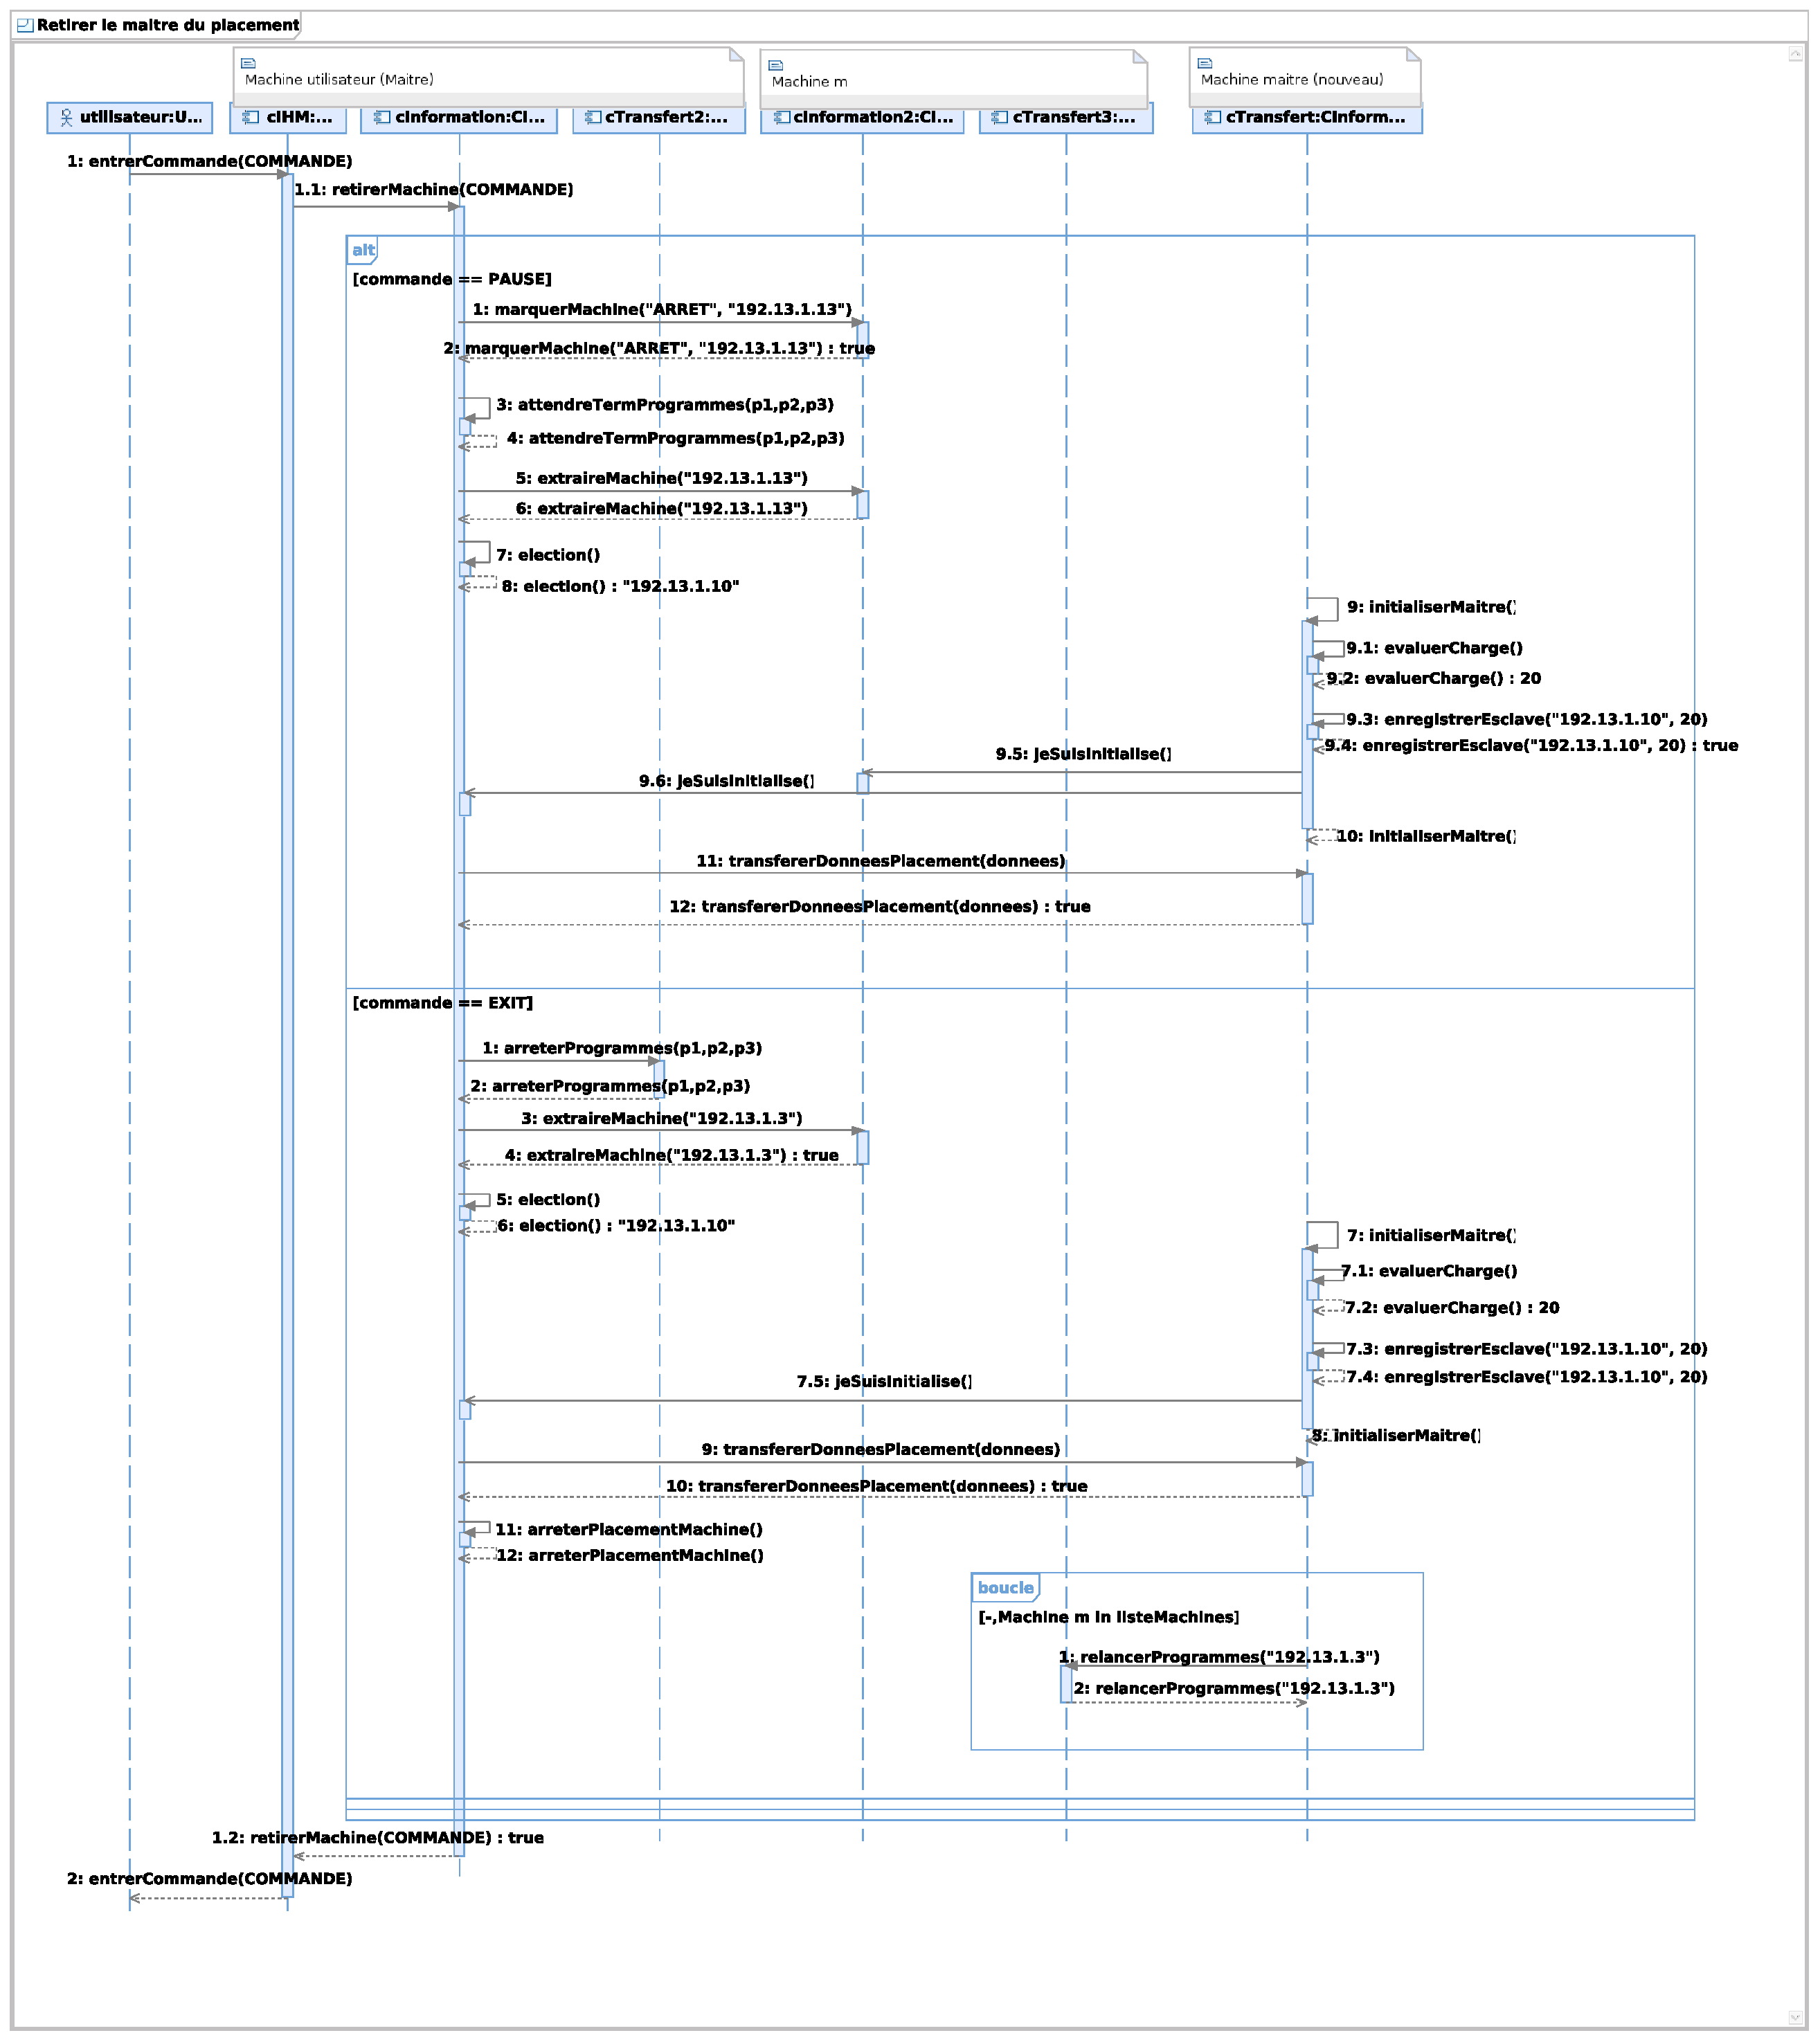
\includegraphics[width=\textwidth]{img/analyse_DSseqretirerMaitre.pdf}
    \caption{Diagramme de séquence -- Cas Retirer la machine maître} 
  \end{figure}
  
  \begin{figure}[h!]
    \centering
    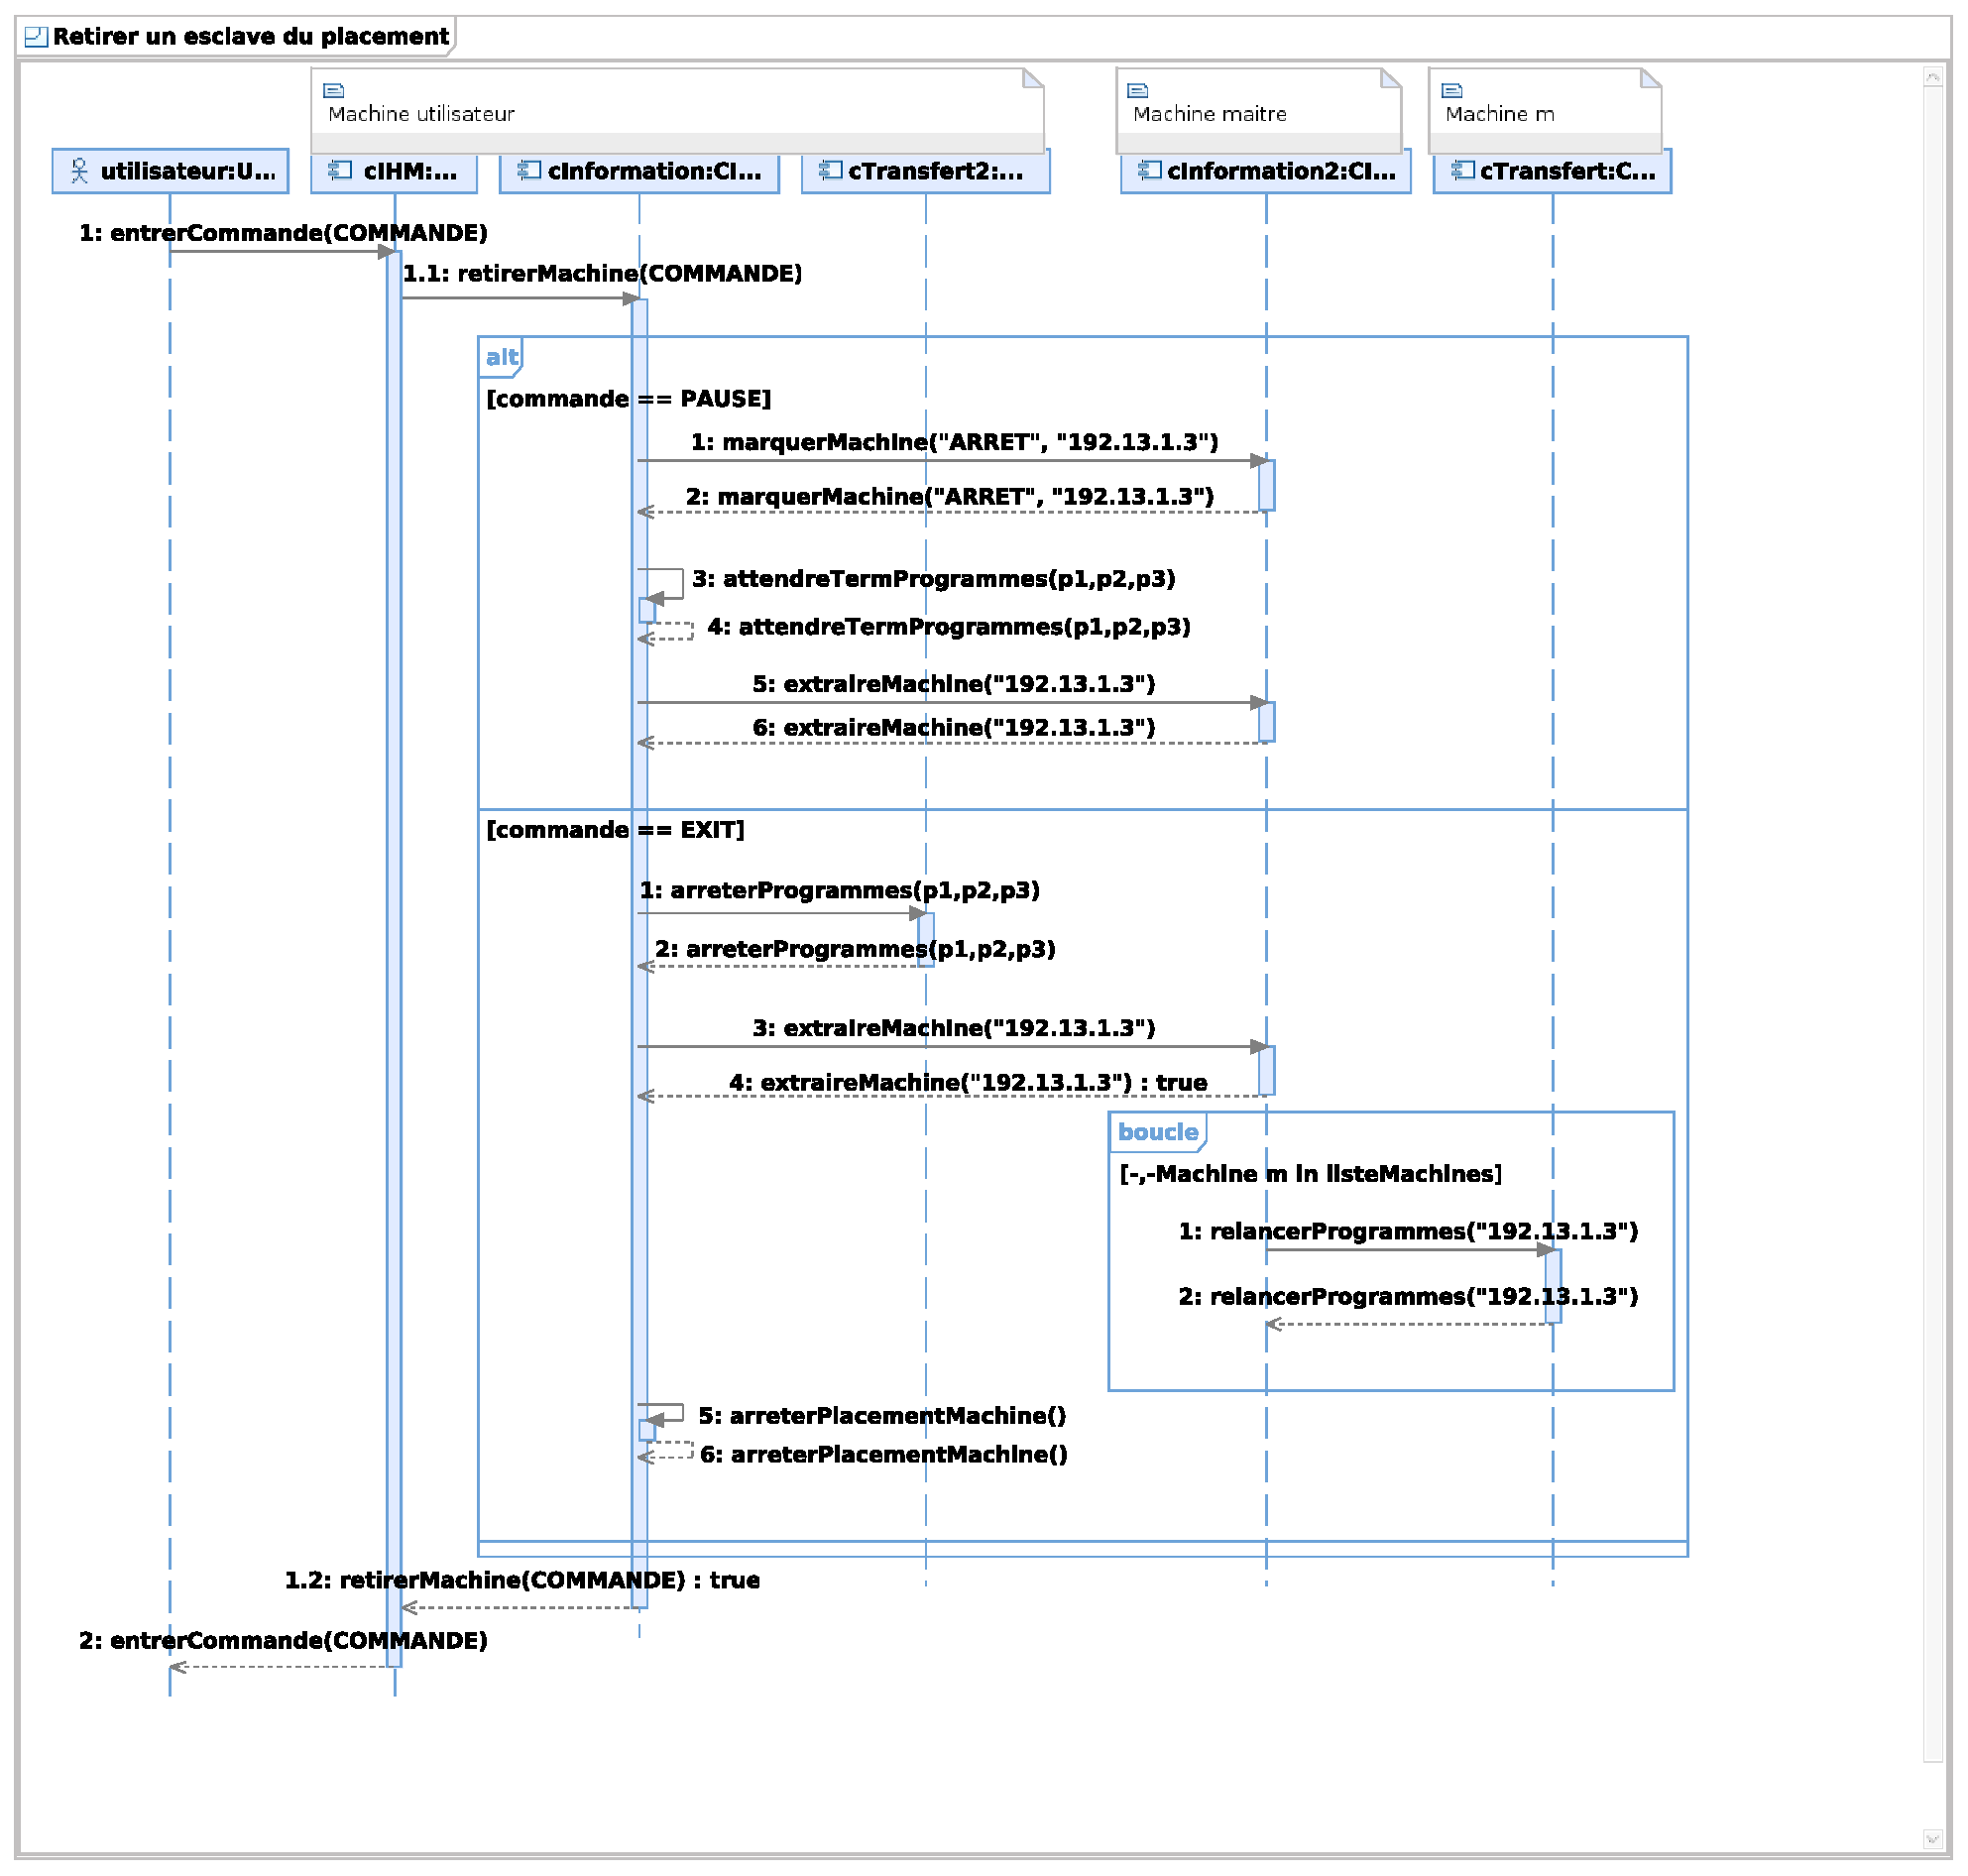
\includegraphics[width=\textwidth]{img/analyse_DSseqretireresclave.pdf}
    \caption{Diagramme de séquence -- Cas Retirer une machine esclave}
  \end{figure}

    \paragraph{Description}Décrire les étapes permettant à un 
      utilisateur de retirer sa machine du placement réparti.
      \begin{description}
        \item[Acteur principal] Utilisateur
        \item[Acteur secondaire] Aucun
        \item[Séquence] le cas d'utilisation commence lorsqu'un 
          utilisateur entre une commande de sortie (PAUSE, EXIT) du
          placement réparti sur sa machine
        \item[Pré-conditions] : La machine doit être une machine intégrée au placement
    \end{description}
    \paragraph{Scénario nominal} : Sortie d'un esclave sans forcer son arrêt
        \begin{enumerate}
          \item L'utilisateur entre la commande de sortie « PAUSE » et valide
          \item Le système vérifie la commande
          \item Le système marque la machine de l'utilisateur afin d'éviter l'exécution à distance de
              nouveaux programmes sur celle-ci
          \item Le système attend la terminaison des programmes exécutes à distance (en cours) sur la
              machine de l'utilisateur
          \item Le système extrait le données (identifiant, charge locale) de la machine des données du
              placement (données présentes sur le maitre)
          \item Le système revient à l'interface d'accueil du placement sur la machine de l'utilisateur
        \end{enumerate}
    \paragraph{Alternatives}
    A1 : Sortie d'un esclave en forçant son arrêt immédiat
            Enchainement démarre au début de la séquence nominale
        \begin{enumerate}
          \item L'utilisateur entre la commande de sortie « EXIT » et valide
          \item Le système vérifie la commande
          \item Le système arrête les programmes exécutés à distance sur la machine de l'utilisateur
          \item Le système extrait le données (identifiant, charge locale) de la machine des données du
              placement (données présentes sur le maitre)
          \item Le système relance sur chaque site, ses programmes interrompu qui s'exécutaient sur la
              machine retirée (voir cas d'utilisation : exécuter un programme)
        \end{enumerate}
    A2 : Sortie d'un maitre sans forcer son arrêt
        \begin{enumerate}
          \item L'utilisateur entre la commande de sortie « PAUSE » et valide
          \item Le système vérifie la commande
          \item Le système marque le maitre afin d'éviter l'exécution à distance de nouveaux programmes
              sur celle-ci
          \item Le système attend la terminaison des programmes exécutes à distance (en cours) sur le
              maitre de l'utilisateur
          \item Le système extrait le données (identifiant, charge locale) du maitre des données du
              placement (données présentes en locale)
          \item Le système élit un leader comme maitre parmi les esclaves
          \item Le système réinitialise le nouveau maitre élu
          \item Le système transfère les données du placement vers le nouveau maitre
          \item Le système informe les esclaves que le nouveau maitre est prêt à recevoir des requêtes
        \end{enumerate}
    A3 : Sortie d'un maitre en forçant son arrêt immédiat
         Enchainement démarre au début de la séquence nominale
        \begin{enumerate}
          \item L'utilisateur entre la commande de sortie « EXIT » et valide
          \item Le système vérifie la commande
          \item Le système arrête les programmes exécutés à distance sur le site maitre
          \item Le système extrait le données (identifiant, charge locale) du maitre des données du
              placement (données présentes en locale)
          \item Le système élit un leader comme maitre parmi les esclaves
          \item Le système réinitialise le nouveau maitre élu
          \item Le système transfère les données du placement vers le nouveau maitre
          \item Le système informe les esclaves que le nouveau maitre est prêt à recevoir des requêtes
          \item Le système relance sur chaque site, ses programmes interrompu qui s'exécutaient sur la
              machine retirée (voir cas d'utilisation : exécuter un programme)
        \end{enumerate}
    A4 : La commande entrée est invalide
         Enchainement démarre après le point 1de la séquence nominale, A1, A2 ou A3
        \begin{enumerate}
        \setcounter{enumi}{2}
          \item Le système indique à l'utilisateur que la commande est incorrectes
         La séquence nominale, A1, A2 ou A3 reprend au point 1
        \end{enumerate}
    A5 : la machine n'a pas de programme en cours d'exécution
         Enchainement 3, 4 de la séquence nominale, A2 ne sont plus considérés
    \paragraph{Exceptions}
    E1 : Problème communication entre machine source et cible
         L'enchainement démarre au point 5 de la séquence A1
            Après trois tentatives sans acquittement, le système abandonne (la suite sera gérée par la
            gestion de pannes)
    \paragraph{Post-conditions}
            Le système a retiré les informations suivantes :
                   - l'identifiant et la charge locale (retirés du placement réparti) de la machine retirée

  \subsubsection{Cas Superviser}

  \begin{figure}[h!]
    \centering
    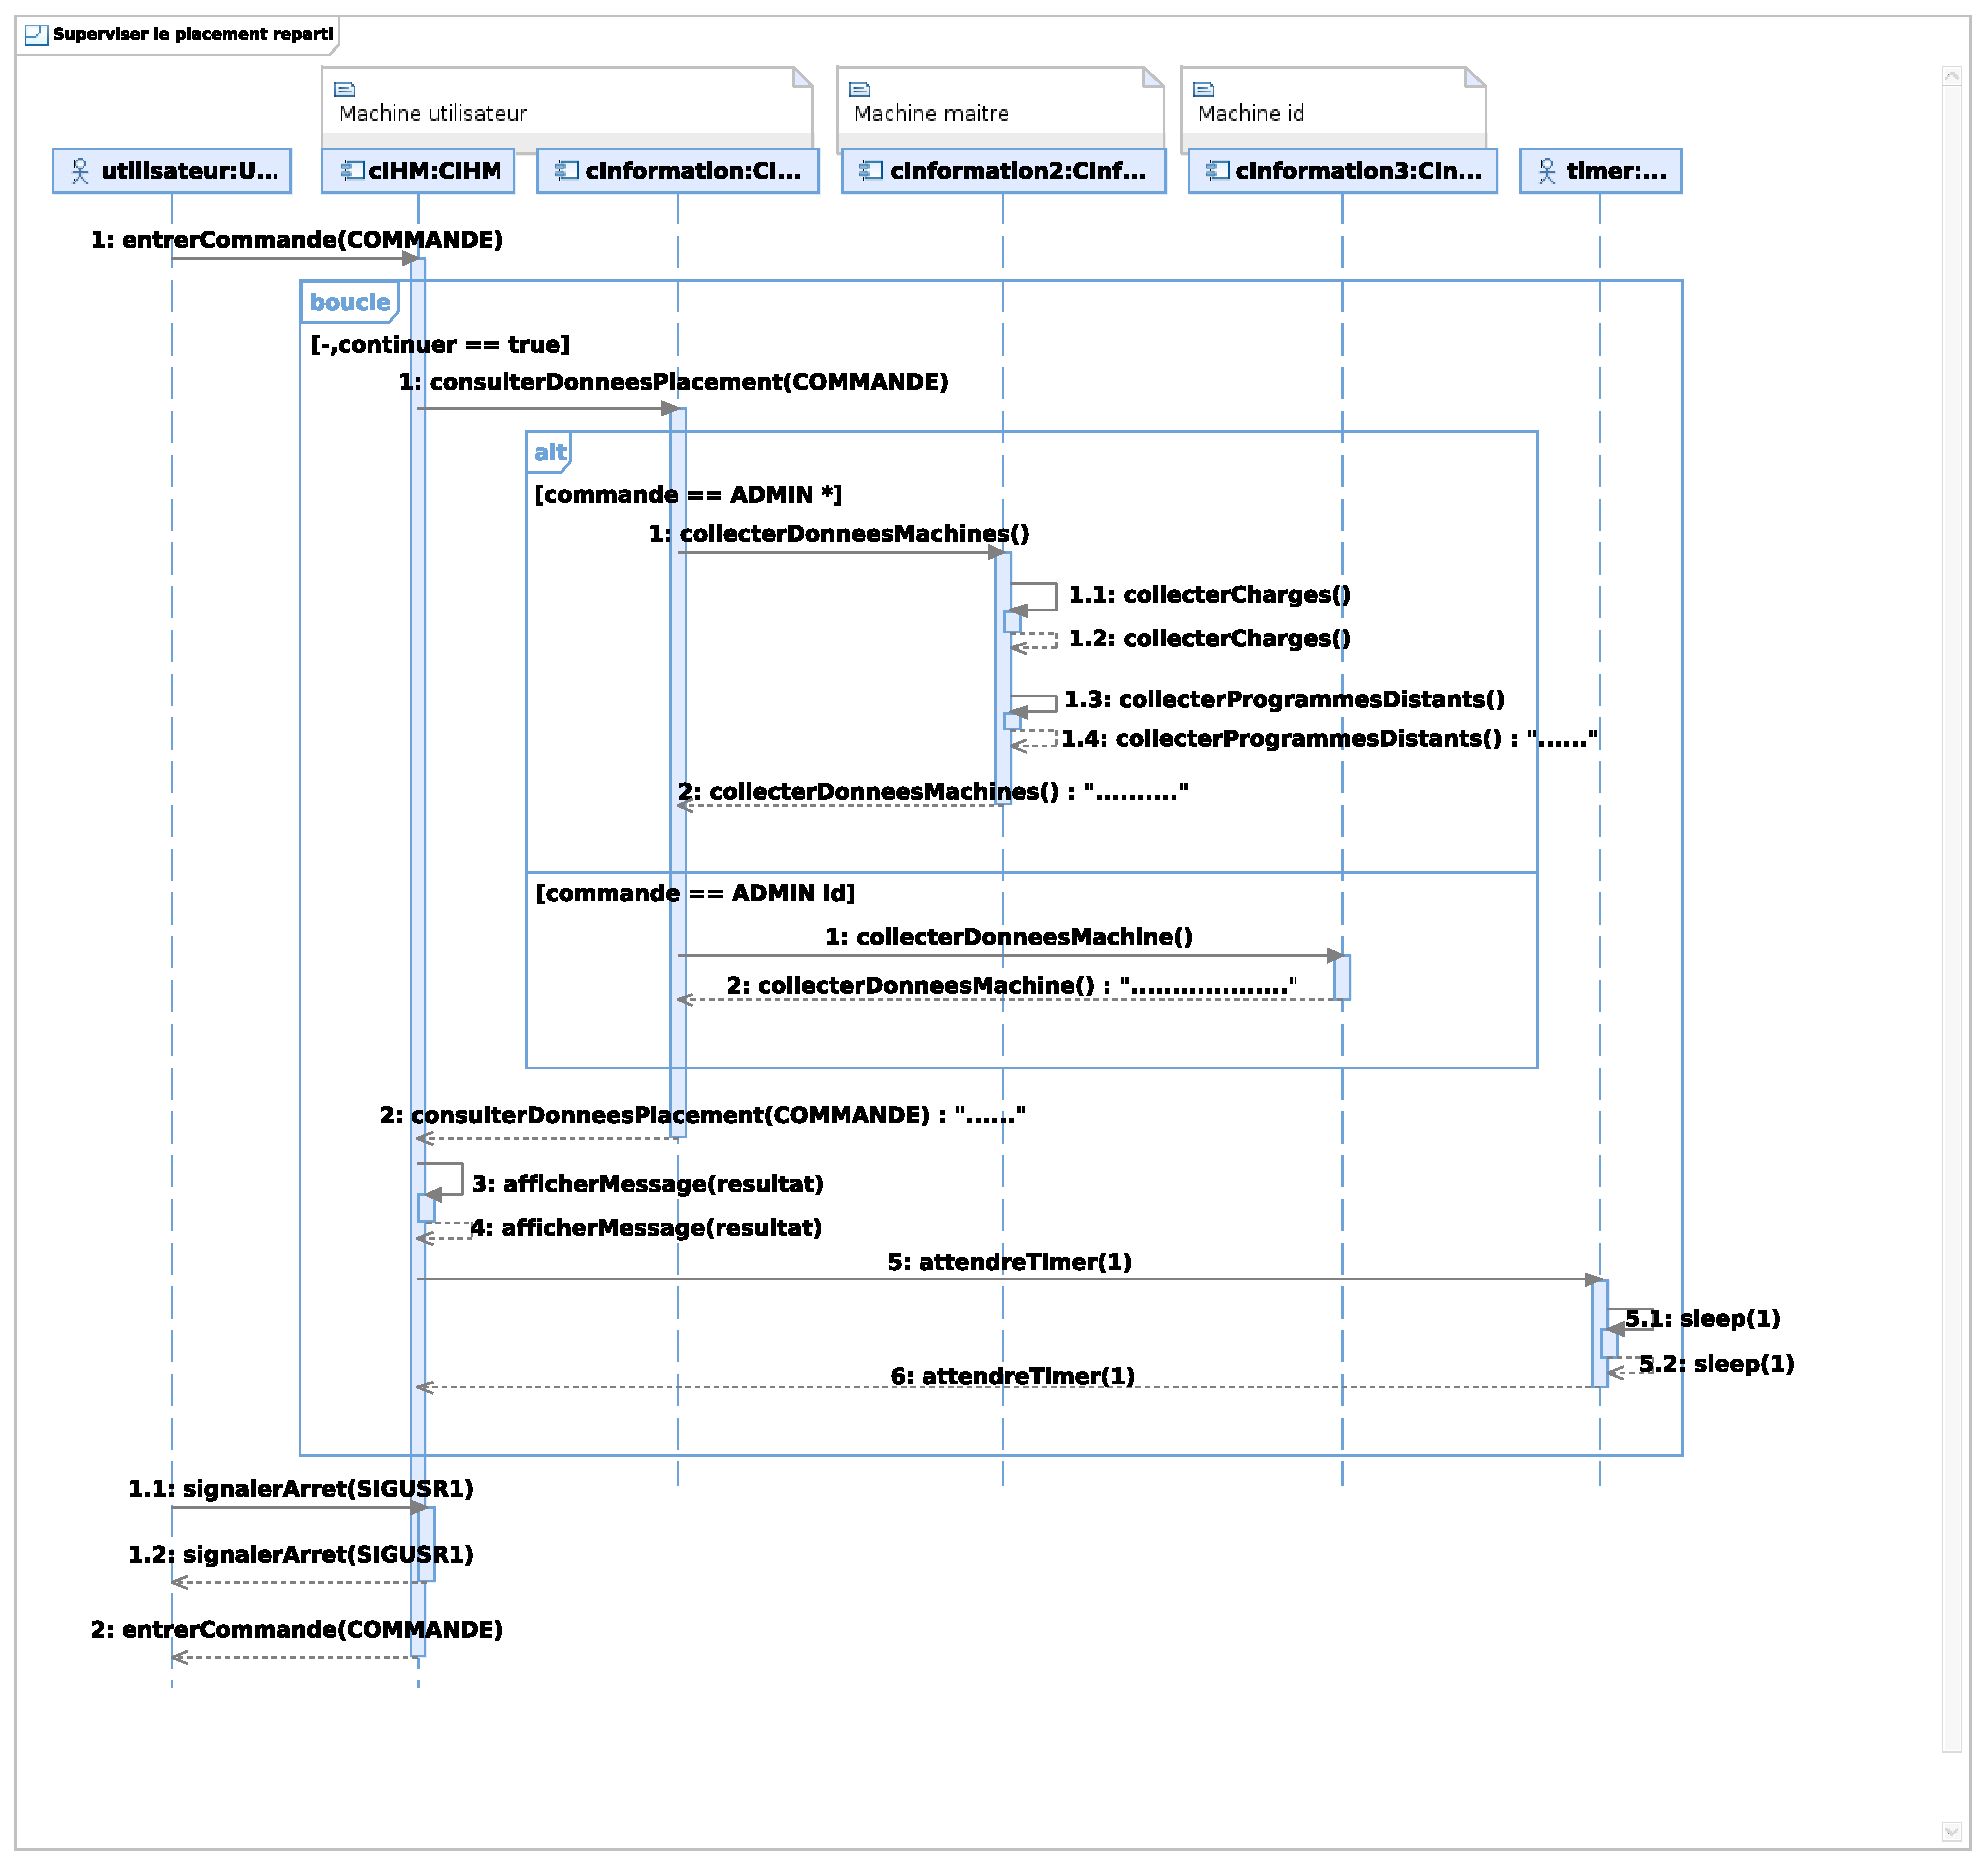
\includegraphics[scale=0.45]{img/analyse_DSseqsuperviser.pdf}
    \caption{Diagramme de séquence -- Cas Superviser le placement réparti}
  \end{figure}

    \paragraph{Description} Décrire les étapes permettant à un utilisateur
      de visualiser les charges locales et les programmes exécutés à
      distance de tous les sites du placement afin de prendre des décisions
      (retrait, ajout de sa machine ou limiter le nombre de programmes
      distantes exécutés sur sa machine, ...).
      \begin{description}
        \item[Acteur principale] : Utilisateur,
        \item[Acteur secondaire] : Timer (traitement périodique)
        \item[Séquence] : le cas d'utilisation commence lorsque l'utilisateur entre la commande « ADMIN *»
        (Tous les sites) ou « ADMIN identifiant » (identifiant d'un site donnée participant au placement).
        \item[Pré-conditions] : le placement réparti de la machine de l'utilisateur doit être au moins démarré.
      \end{description}
    \paragraph{Scénario nominal}
        \begin{enumerate}
          \item L'utilisateur entre la commande « ADMIN * » pour avoir des informations sur tous les sites
             du placement.
          \item Le système récolte l'identifiant, la charge, les programme exécutés à distance de chaque site
             du placement réparti.
          \item Le système affiche l'identifiant, la charge, les programmes exécutés à distance de chaque site
             du placement.
          \item Le Timer maintient à jour la récolte et l'affichage périodiquement pour garder les données
             fraiches.
          \item L'utilisateur ferme l'affichage
          \item Le système revient à l'invite des commandes
        \end{enumerate}
    \paragraph{Alternatives}
    A1 : L'utilisateur entre la commande « ADMIN identifiant » pour avoir les informations d'une
    machine donnée.
         Enchainement démarre au début de la séquence nominale
         \begin{enumerate}
           \item L'utilisateur entre la commande « ADMIN identifiant » d'une machine
           \item Le système récolte l'identifiant, la charge, les programmes exécutés à distance de la machine
           \item Le système affiche les informations suivantes de la machine donnée :
               - son identifiant,
               - sa charge,
               - ses programmes exécutés à distance,
               - les programmes d'autres sites qu'il exécute
          \end{enumerate}
         La séquence nominale reprend au point 4
    \paragraph{Exceptions}
     E1 : la commande est « ADMIN identifiant » et le site n'est pas intégré au placement.
          Enchainement démarre après le point 1 de la séquence A1
          \begin{enumerate}
          \item le système indique l’erreur à l'utilisateur et revient à l'invite de commandes
          La séquence nominale reprend au début
          \end{enumerate}

  \subsubsection{Cas Gérer une panne}

  \begin{figure}[h!]
    \centering
    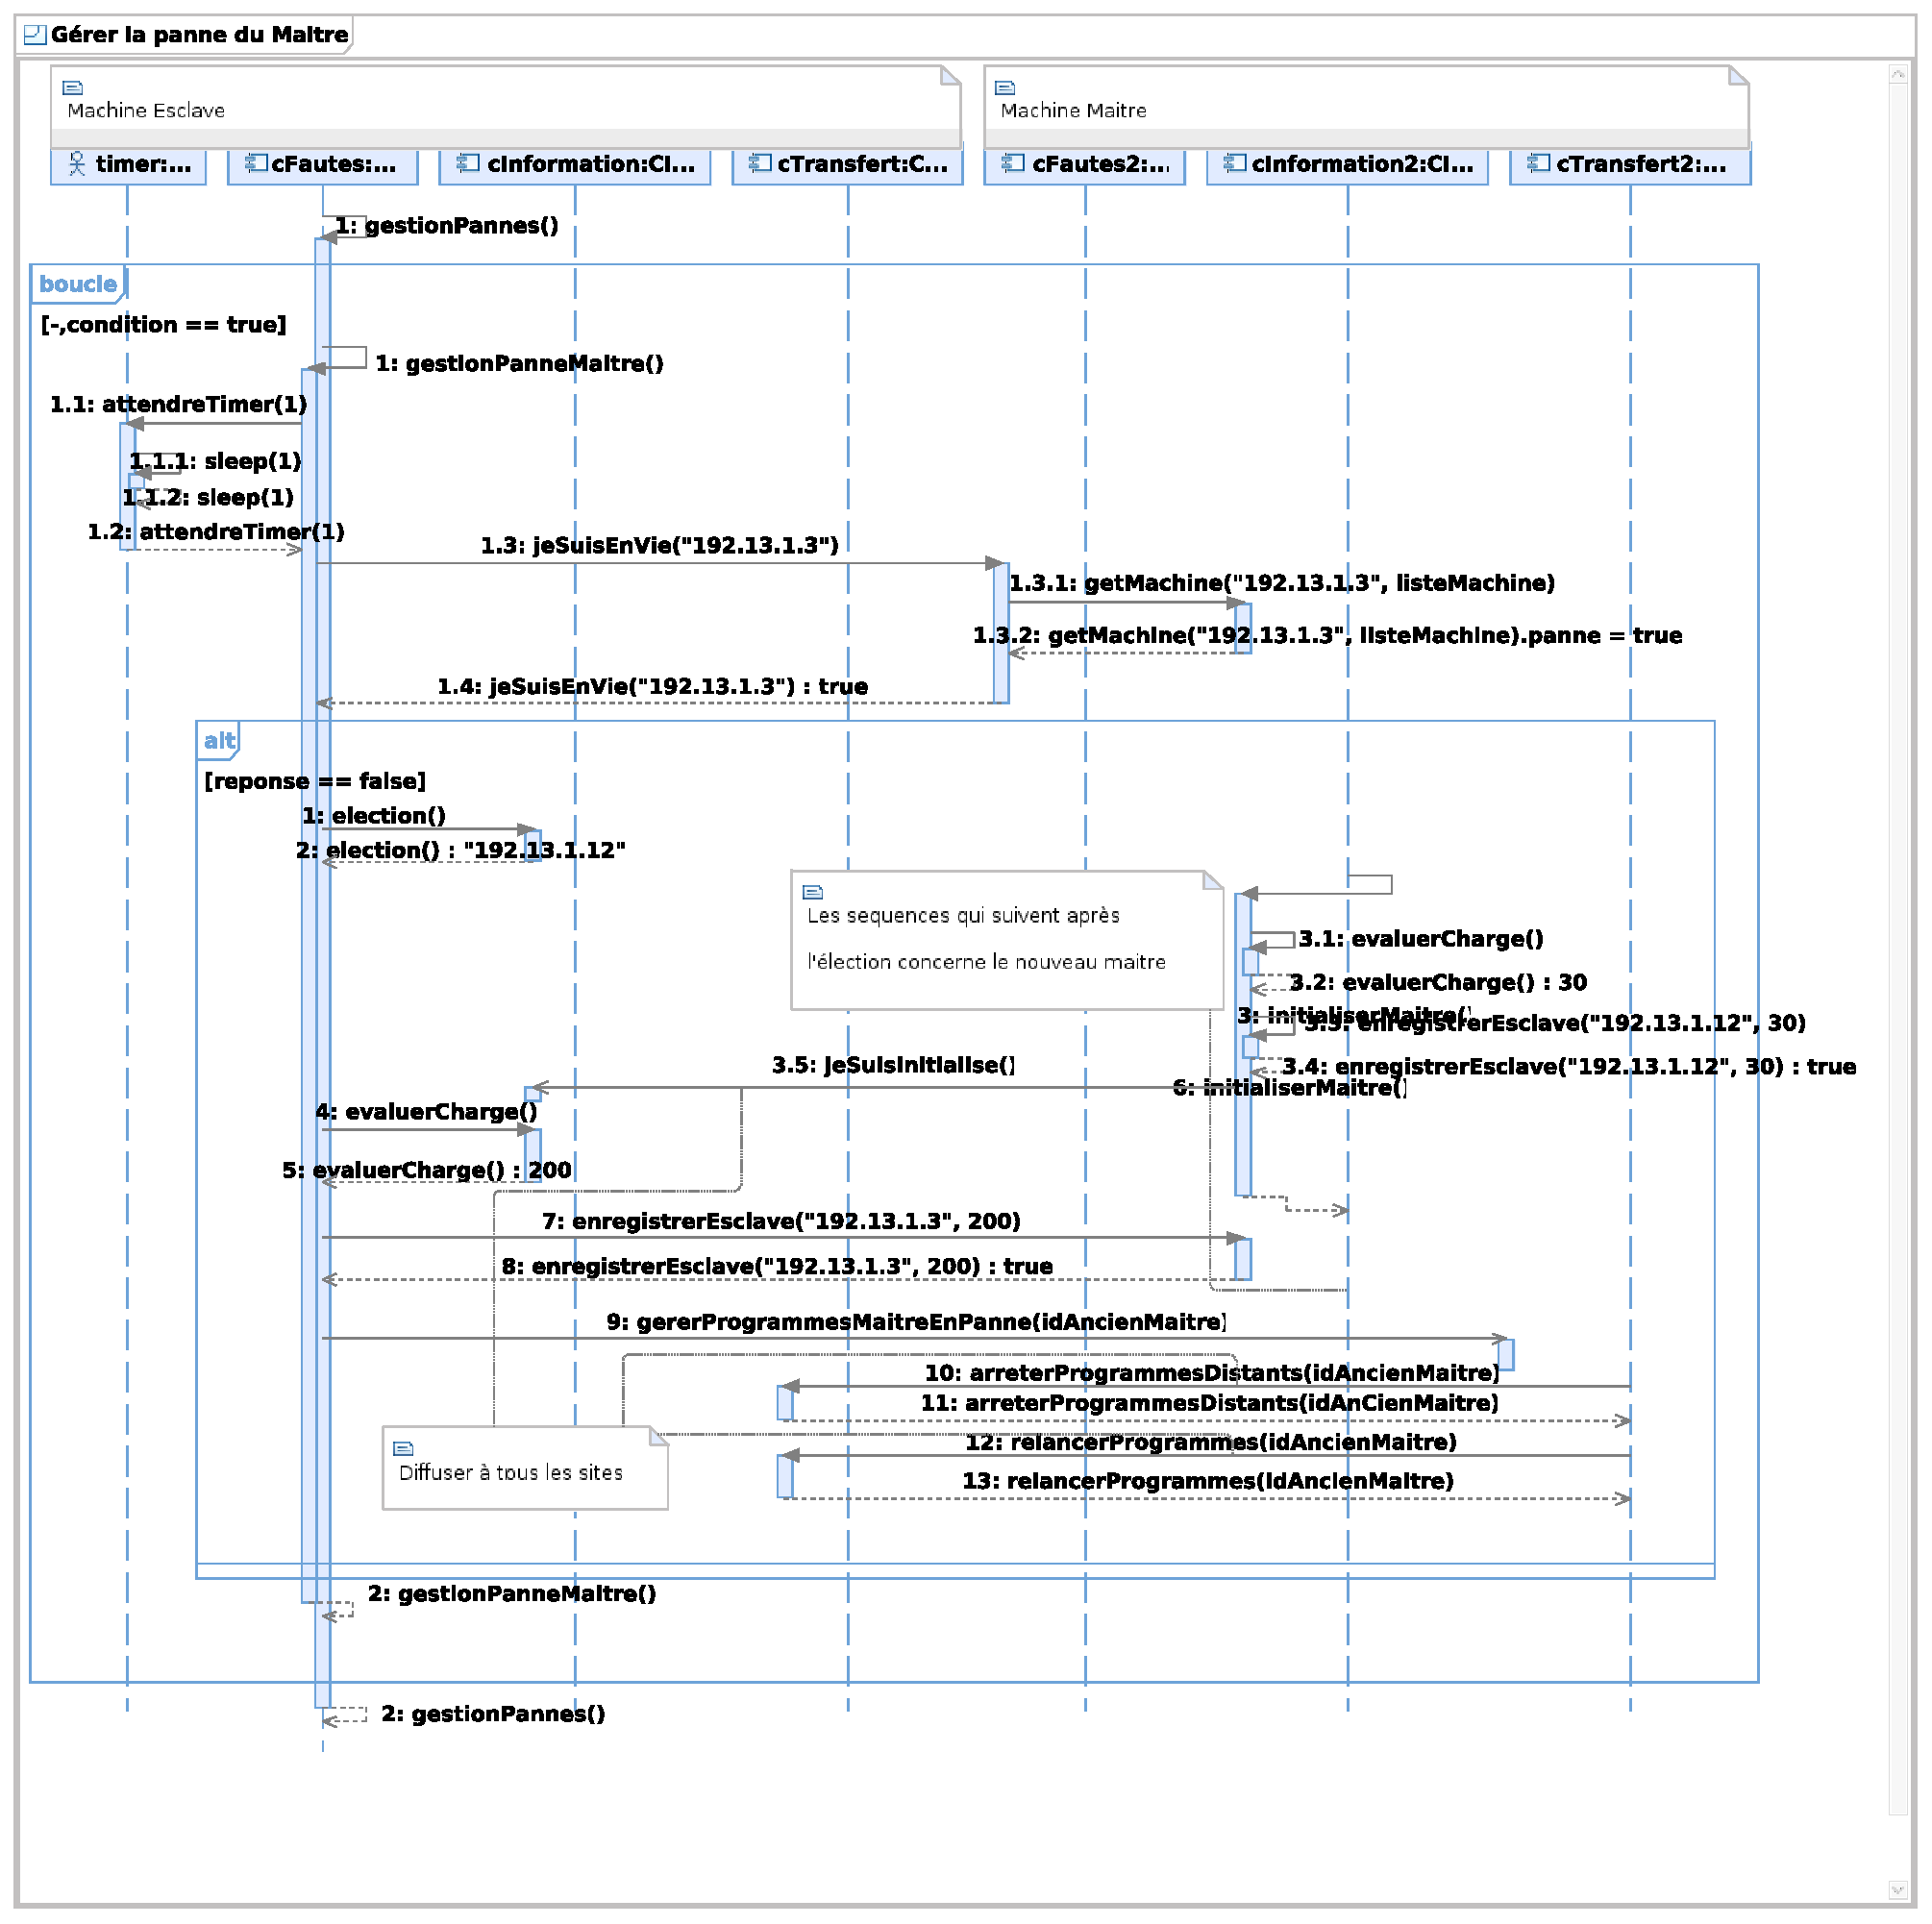
\includegraphics[scale=0.4]{img/analyse_DSseqpanneMaitre.pdf}
    \caption{Diagramme de séquence -- Cas Gestion de panne d'un maître}
  \end{figure}
  
  \begin{figure}[h!]
    \centering
    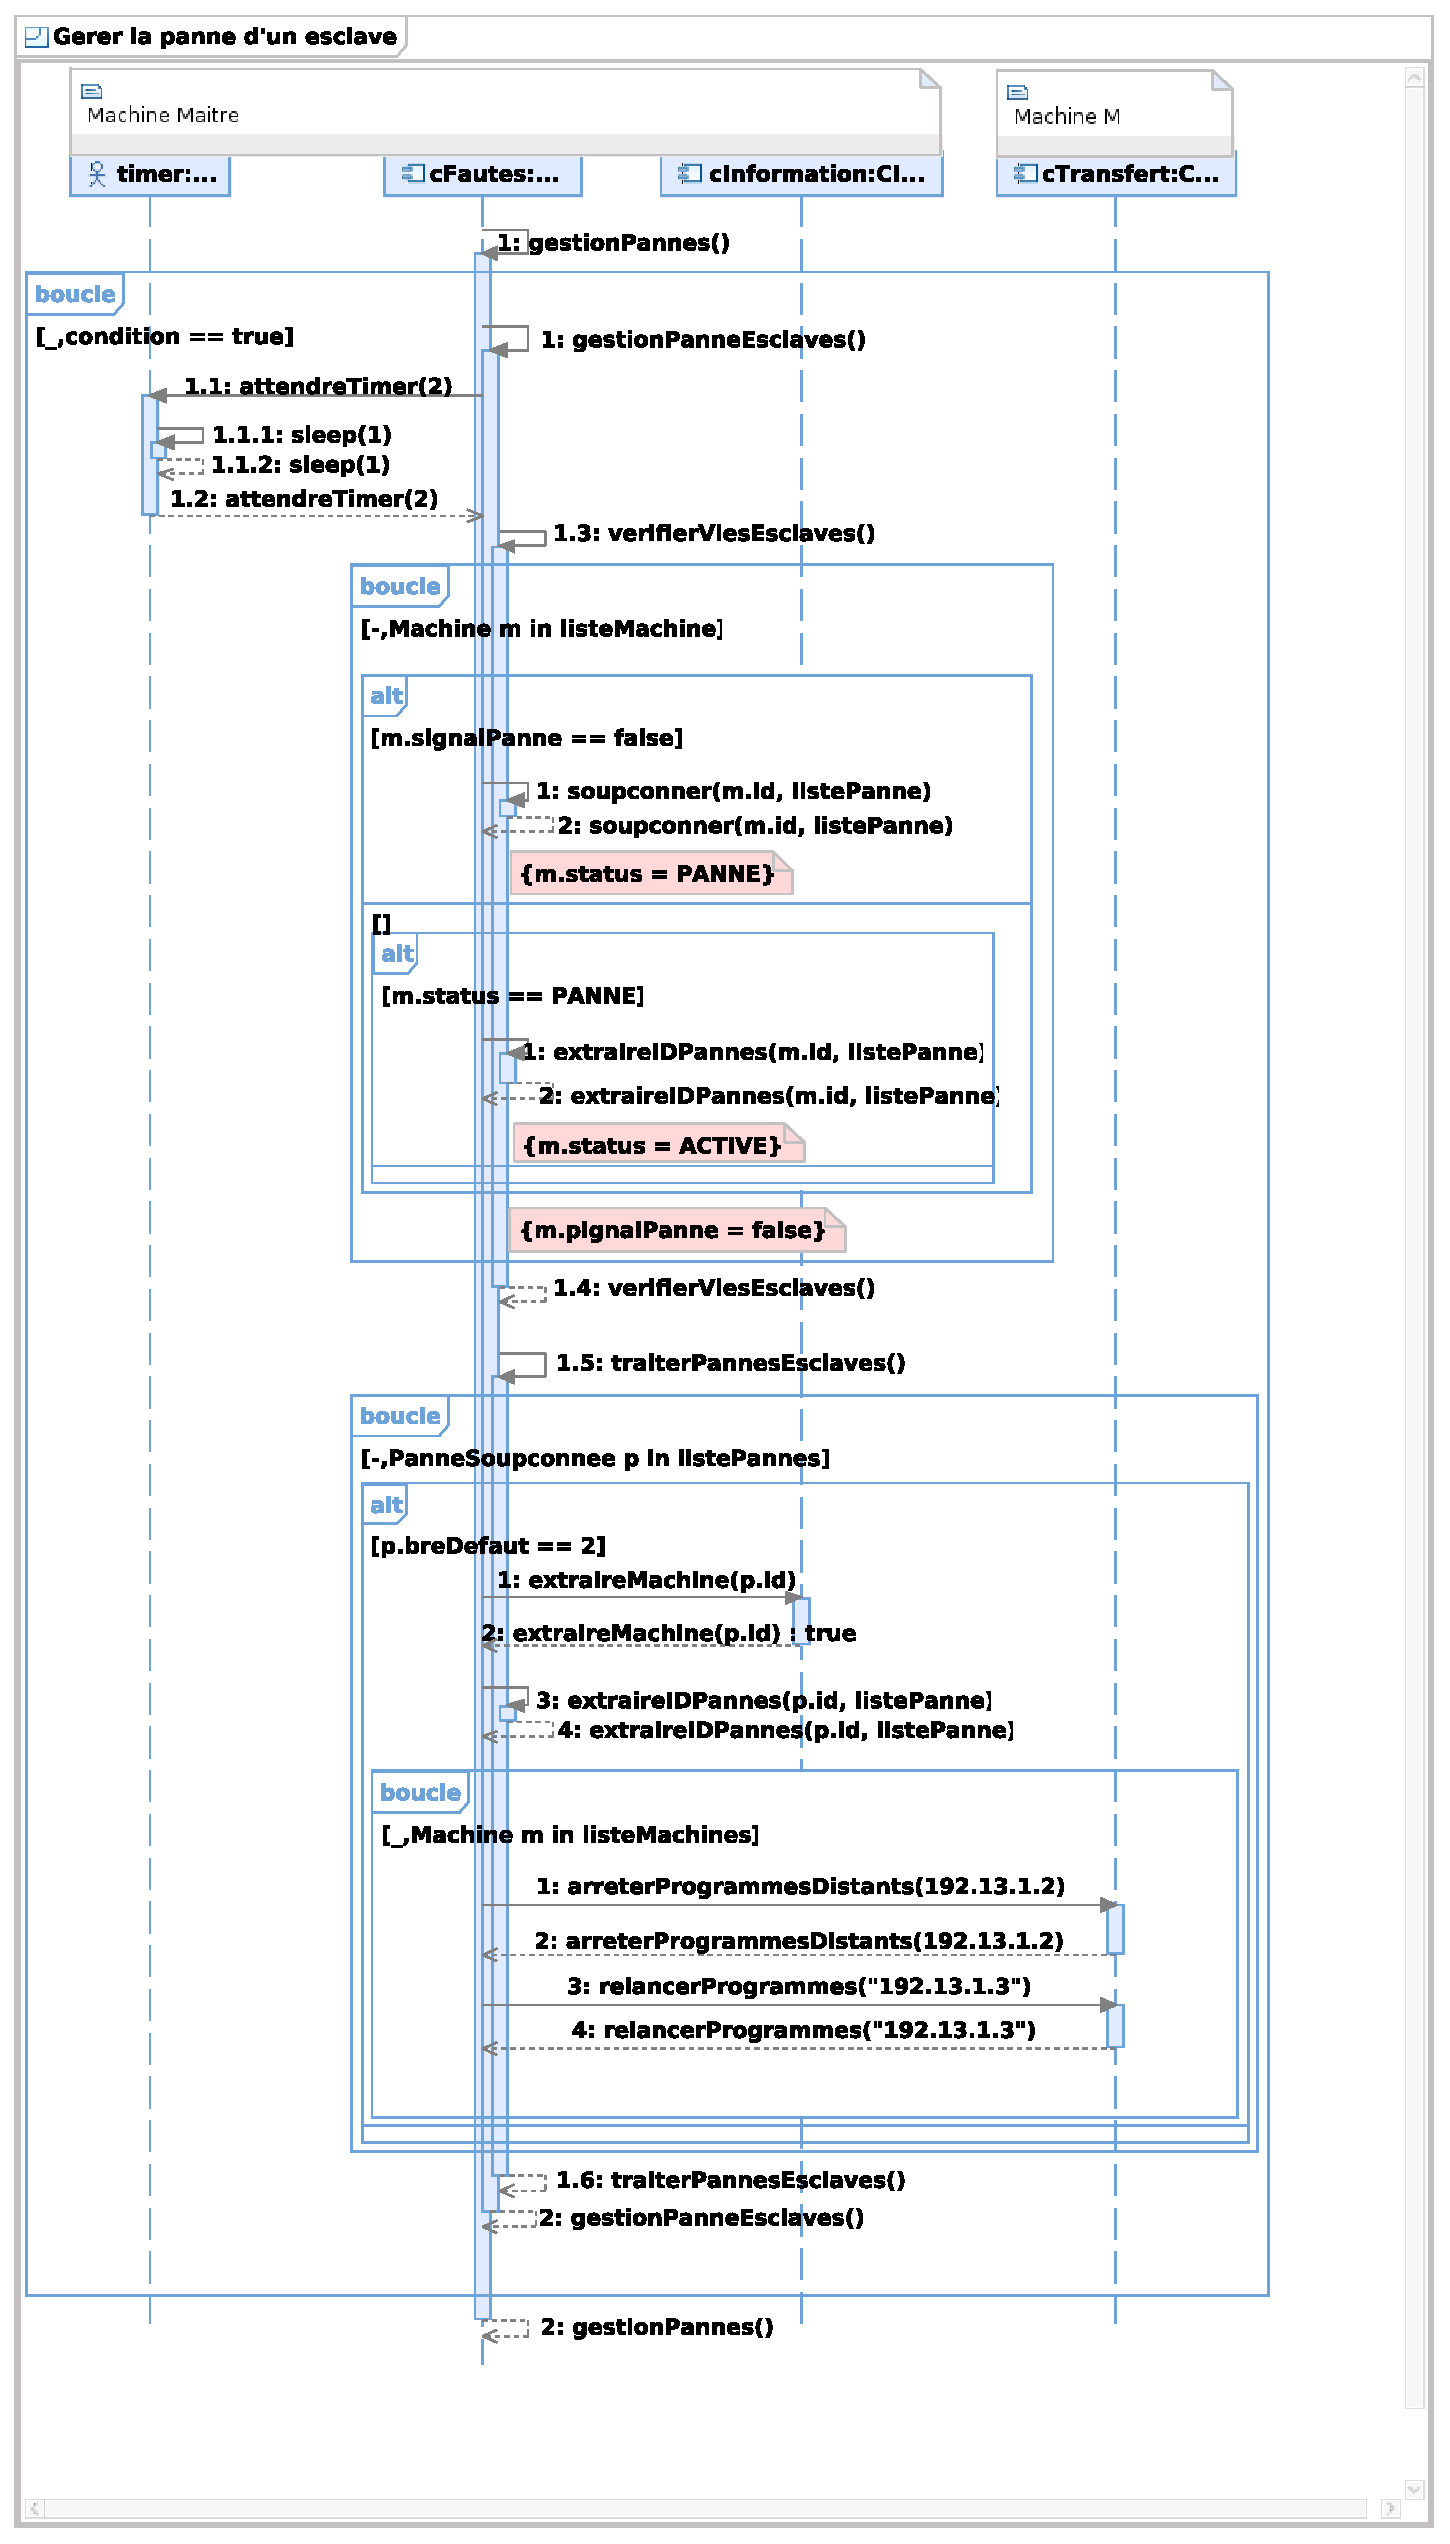
\includegraphics[scale=0.409]{img/analyse_DSseqpanneEsclave.pdf}
    \caption{Diagramme de séquence -- Cas Gestion de panne d'un esclave}
  \end{figure}

    \paragraph{Description} : Décrire les étapes permettant de gérer une machine du placement en panne détectée
    par un traitement périodique.
    \begin{description}
      \item[Acteur principal] Timer (Traitement périodique)
      \item[Acteur secondaire] Aucun
      \item[Séquence] le cas d'utilisation démarre lorsque la panne d'une machine est détectée.
      \item[Pré-conditions] la machine en panne doit être une machine intégrée au placement
    \end{description}
    \paragraph{Scénario nominale} : (Esclave) Avant de tomber en panne, le site avait des programmes exécutés à
    distance
        \begin{enumerate}
          \item Le Timer vérifie si une machine n'est pas en panne
          \item Le Timer détecte une panne d'une machine
          \item Le système vérifie si c'est un esclave ou le maitre en panne
          \item Le système extrait le données (identifiant, charge locale) de la machine des données du
              placement (données présentes sur le maitre)
          \item Le système demande aux autres sites d'arrêter ses programmes exécutant à distance
          \item Le système relance sur chaque machine, ses programmes interrompu sur la machine en
              panne (voir cas d'utilisation exécuter un programme)
        \end{enumerate}
    \paragraph{Alternatives}
    A1 : (Maitre) Avant de tomber en panne, le maitre avait des programmes exécutés à distance
         Enchainement démarre après le point 3 de la séquence nominale
        \begin{enumerate}
        \setcounter{enumi}{3}
          \item Le système demande aux autres sites d'arrêter les programmes du maitre exécutant à
              distance
          \item Le système élit un leader comme maitre parmi les esclaves
          \item Le système réinitialise le nouveau maitre élu
          \item Le système récolte et enregistre l'identifiant et la charge de chaque site du placement sur le
              maitre
          \item Le système relance sur chaque machine, ses programmes interrompu sur la machine maitre
              en panne (voir cas d'utilisation exécuter un programme)
        \end{enumerate}
    A2 : Avant de tomber en panne, la machine n'exécutait pas de programmes pour d'autres
         L'enchainement du point 6 de la séquence nominale ou 8 de la séquence A1 est ignoré
    A2 : Avant de tomber en panne la machine n'exécutait pas des programmes sur d'autres
         L'enchainement du point 5 de la séquence nominale ou 4 de la séquence A1 est ignoré
    A3 : Le Timer ne détecte pas de panne
       L'enchainement des points 3, 4, 5, 6, 7, 8 sont ignorés
    \paragraph{Post-conditions}
            La machine n'est plus dans le placement et le système a retiré les informations suivantes :
                – cas esclave : les programmes exécutés à distance du site en panne


%%%
\subsection{Données métier}
  
  \noindent Côté esclave :
    \begin{itemize}
      \item Le maître
      \item Les programmes exportés (ses programmes qui sont en train de s'exécuter à distance)
      \item Les programmes importés (les programmes des autres sites qui s'exécutent sur lui)
     \end{itemize}
        
   \noindent Côté maître :
     \begin{itemize}
       \item Tous les esclaves
       \item Les programmes exportés
       \item Les programmes importés
       \item La liste des sites soupçonnes d'être en panne
      \end{itemize} 
        
\subsection{Diagramme de classe}
  Etant donnée que notre projet a pour contrainte d'étre écrit en C ce 
  diagramme représente les structures de données à définir dans notre
  application.

     \begin{figure}[h!]
       \centering
       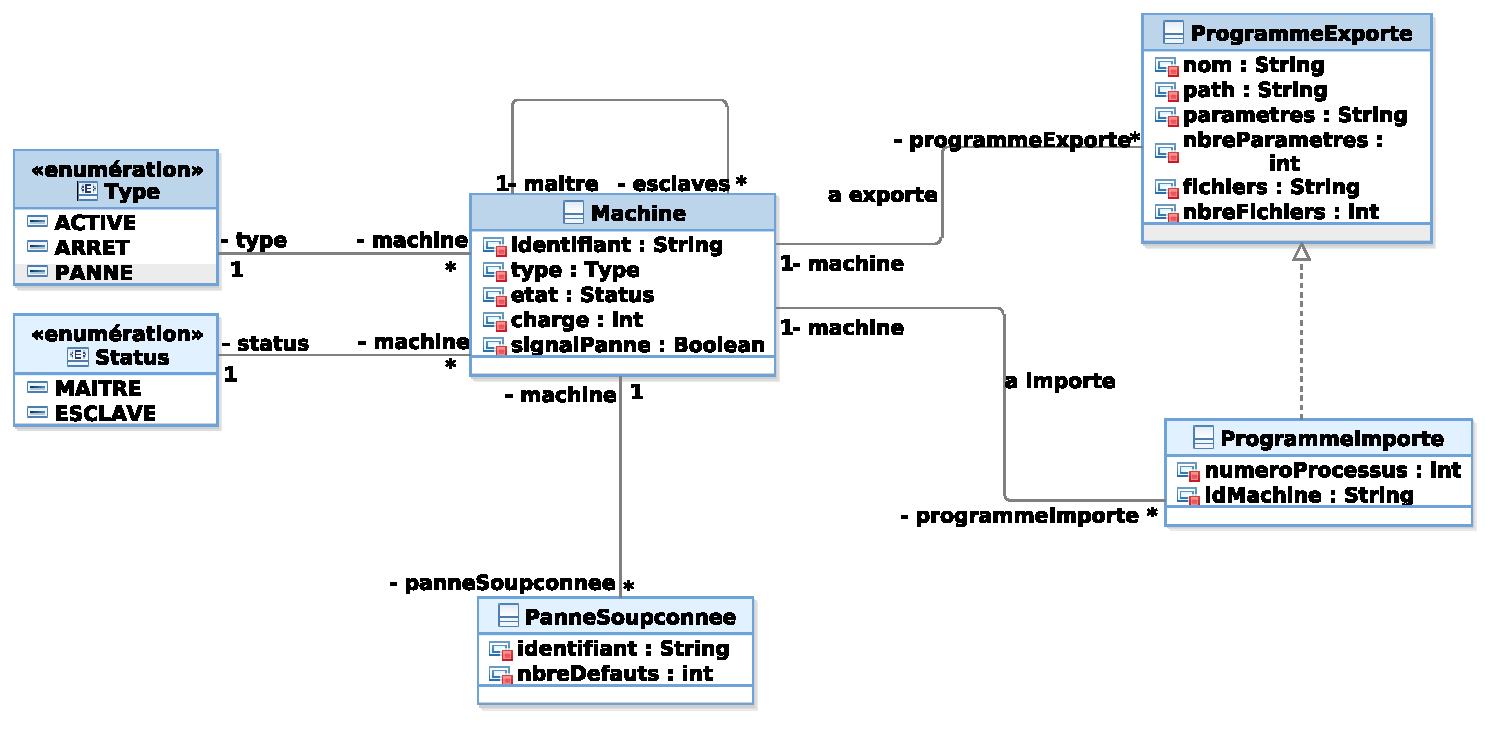
\includegraphics[width=\textwidth]{img/analyse_dcl.pdf}
       \caption{Diagramme de classe}
     \end{figure}
\newpage

\subsection{Diagramme de composant}

  \begin{figure}[h!]
    \centering
    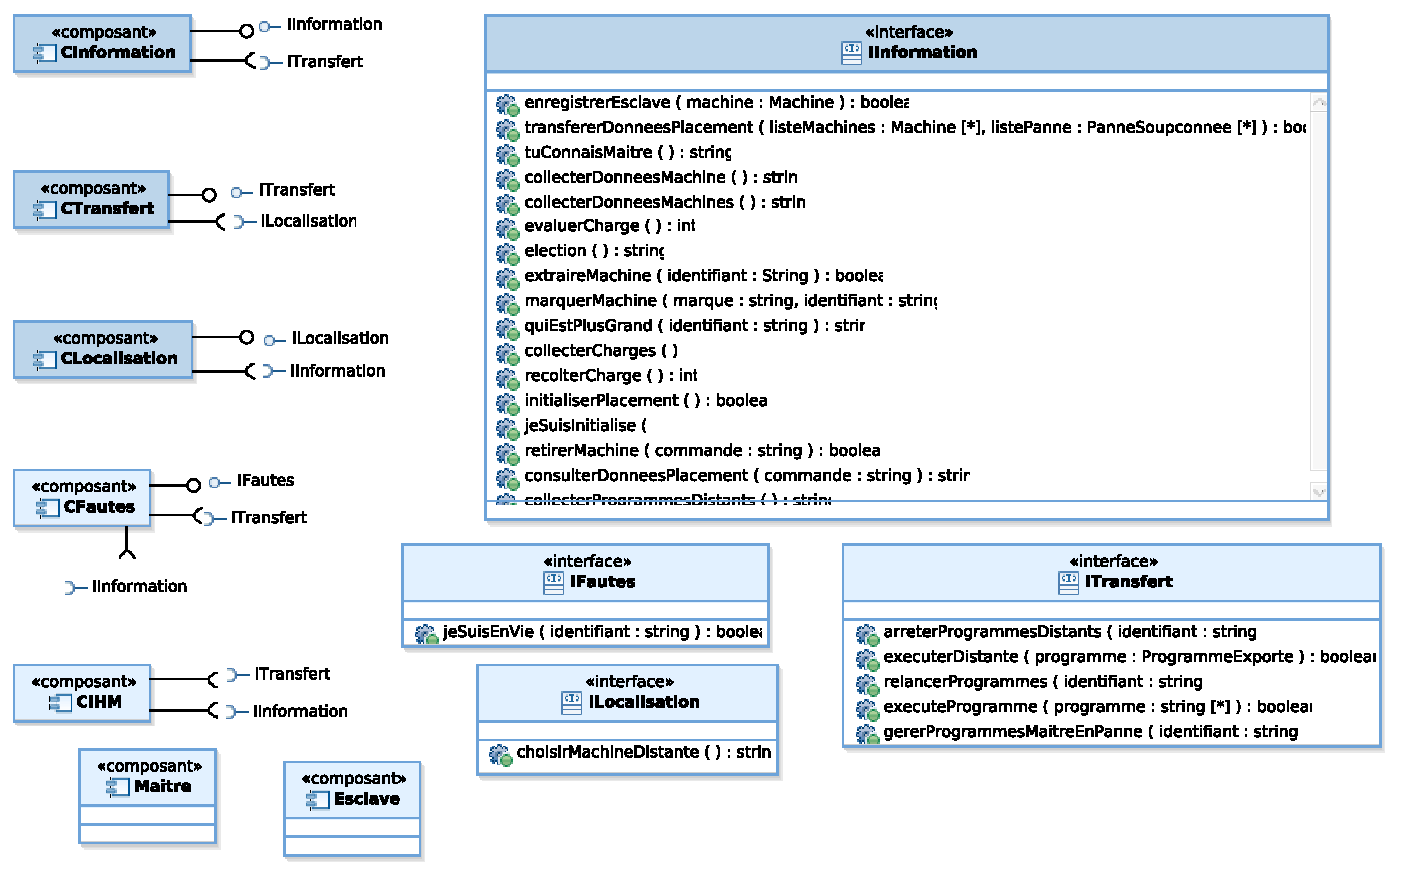
\includegraphics[angle=270,width=0.8\textwidth]{img/analyse_DiagrammeComposant.pdf}
    \caption{Diagramme de composant}
  \end{figure}
